% Chapter Title Page
\clearpage
\thispagestyle{empty} 
\begin{center}
    \vspace*{\fill} 
    \Huge \textbf{Chapter 6} \\
    \Huge \textbf{Asymmetric Encryption} 
    \vspace*{\fill}
\end{center}
\clearpage
\chapter{Asymmetric Encryption}

\section{Definition}
Public-key cryptography, also known as asymmetric cryptography, uses two separate keys for encryption and decryption. This contrasts with symmetric encryption, which uses only one key.

\section{Ingredients of Asymmetric Encryption}
\begin{figure}
    \centering
    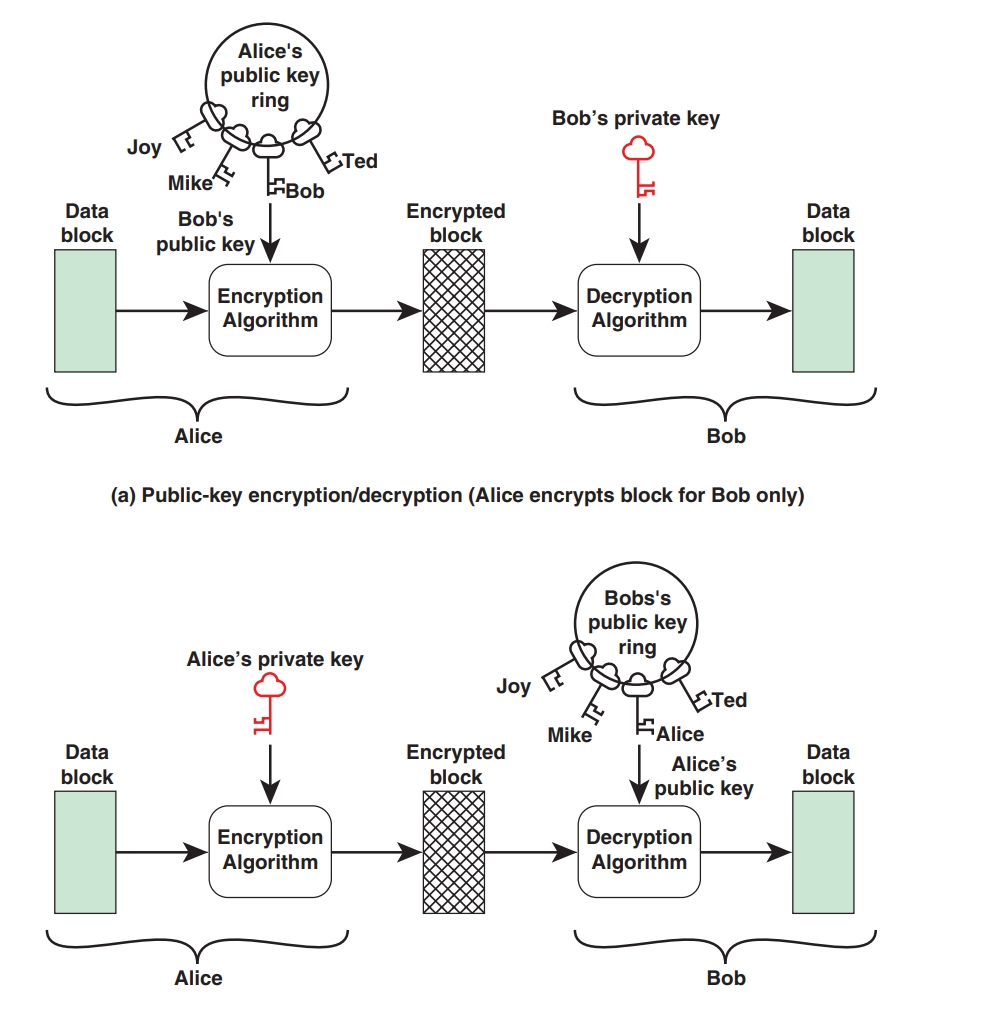
\includegraphics[width=1\linewidth]{Data_Privacy_and_Cryptography/Figures/model of asymmetric crypto.jpeg}
    \caption{Model of Asymmetric Cryptosystem}
    \label{fig:asymmetric}
\end{figure}
\begin{itemize}
    \item \textbf{Plaintext:} The readable message or data block input into the encryption algorithm.
    \item \textbf{Encryption Algorithm:} Performs various transformations on the plaintext using a key.
    \item \textbf{Public Key and Private Key:} A pair of keys selected such that if one key is used for encryption, the other is used for decryption. The transformations depend on the key used.
    \item \textbf{Ciphertext:} The scrambled block produced as output, depending on the plaintext and the key used.
    \item \textbf{Decryption Algorithm:} The inverse of the encryption algorithm, it accepts the ciphertext and the matching key to produce the original plaintext.
\end{itemize}

\section{Process of Asymmetric Encryption}

\begin{itemize}
    \item \textbf{Key Generation:} Each user generates a pair of keys (public and private) for encryption and decryption.
    \item \textbf{Public Key Sharing:} One of the keys (public key) is placed in a public register or accessible file, while the companion key (private key) is kept secret.
    \item \textbf{Encryption:} If Alice wants to send a confidential message to Bob, she encrypts the message using Bob’s public key.
    \item \textbf{Decryption:} Bob decrypts the message using his private key. No one else can decrypt the message because only Bob knows his private key.
\end{itemize}

\section{Comparison with Symmetric Encryption}
\begin{table}[h!]
    \centering
\begin{tabular}{|p{6.5cm}|p{6.5cm}|}
\hline
\textbf{Symmetric Encryption} & \textbf{Asymmetric Encryption} \\
\hline
Uses the same algorithm with the same secret key for encryption and decryption. & Uses one algorithm for encryption and a related algorithm for decryption, with a pair of keys (public and private). \\
\hline
Sender and receiver must share the algorithm and the secret key. & Sender and receiver must each have a unique public/private key pair. \\
\hline
Key must be kept secret. & Private key must be kept secret. \\
\hline
Algorithm plus samples of ciphertext must be insufficient to determine the key. & Algorithm plus public key plus samples of ciphertext must be insufficient to determine the private key. \\
\hline
\end{tabular}
\caption{Symmetric Vs Asymmetric Encryption}
\end{table}
\section{Alternative Uses}

\begin{itemize}
    \item \textbf{Authentication:} 
    \\
    Alice can use her private key to encrypt a message. When Bob decrypts it with Alice’s public key, he can be certain the message came from Alice.
\end{itemize}

\section{Security Considerations}
The security of public-key encryption relies on the strength of the algorithm and the length of the private key. 
\\
Public-key cryptographic algorithms are generally slower than symmetric algorithms and are often limited to small blocks of data, such as a secret key or a hash value.
